\section{Experiments and Results}

\subsection{Implementation Details}
Qwen3-8B embeddings were generated on an NVIDIA RTX\,3090
(124{,}158 patients, $\approx$7\,h per embedding run).
Bio\_ClinicalBERT (110M params) runs on the same GPU at
$\approx$30 min per pass.
CoxPH models were fitted on CPU with \texttt{lifelines} v0.27.
Evaluation used \texttt{scikit-survival} for TD-AUC and IBS.
Code and evaluation scripts are available at [repository URL].

\subsection{Main Results: Representation Axis}

Table~\ref{tab:main} compares the reference configuration for each setting:
Settings 1 and 2 have fixed pipelines; Settings 3 and 4 use Qwen3-8B with
concatenation fusion; Setting 5 uses Qwen3-8B alone (no raw features).

\begin{table}[t]
\centering
\caption{Test-set survival prediction per setting (reference configuration).
         Best values in \textbf{bold}.
         $\uparrow$ higher is better; $\downarrow$ lower is better.}
\label{tab:main}
\begin{tabular}{llccc}
\toprule
Setting & Description & C-index $\uparrow$ & Mean TD-AUC $\uparrow$ & IBS $\downarrow$ \\
\midrule
S1 & Baseline CoxPH (39 features)      & 0.6191 & 0.5999 & 0.1410 \\
S2 & Delphi zero-shot                  & 0.6161 & 0.5984 & 0.1846 \\
S3 & Prose + Qwen + concat             & 0.6156 & \textbf{0.6074} & 0.1409 \\
S4 & Decoupled + Qwen + concat         & \textbf{0.6233} & 0.5991 & 0.1410 \\
S5 & Unified prose, Qwen (no raw)      & 0.6195 & 0.6128 & \textbf{0.1408} \\
\bottomrule
\end{tabular}
\end{table}

\paragraph{Finding 1: Temporal ordering is the critical structural property.}
Setting 4 achieves the best Harrell C-index among the reference configurations (0.6233),
exceeding S1 by $+$0.004 and S3 by $+$0.008.
Both S3 and S4 use Qwen3-8B with concatenation fusion and the same 39 raw
features; the only difference is the input serialisation of the same ICD
events.
Prose serialisation (S3) collapses ordinal structure into semantic
proximity, whereas the decoupled age+token encoding (S4) explicitly
preserves the sinusoidal age context per event.
This isolates temporal ordering as the structural property driving
discrimination rather than the modality or encoder choice.
The absolute C-index differences (0.004--0.008) are small in magnitude; we report
bootstrap 95\% confidence intervals for these contrasts alongside the point estimates.

\paragraph{Finding 2: LLMs can encode numeric structure from prose.}
Setting 5 (unified prose, no raw features) achieves C\,=\,0.6195,
matching S1 (0.6191) while using \emph{no raw numeric features}.
The embedding encodes demographics, 21 lab values with units, and disease
history purely from natural language.
S5 achieves the best calibration (IBS\,=\,0.1408) and strong mean TD-AUC
(0.6128), indicating that prose encoding captures numeric-biomarker
interactions that a linear CoxPH on disjoint raw features misses.

\paragraph{Finding 3: Zero-shot inference has a calibration gap.}
Delphi (S2) achieves C\,=\,0.6161 but substantially worse calibration
(IBS\,=\,0.185 vs.\ $\approx$0.141 for all CoxPH variants).
Its TD-AUC profile is unusual: 0.52 at 9.5\,yr (Table~\ref{tab:horizon})
rising to 0.65 at 19.7\,yr, suggesting chronic-disease priors that align
poorly with near-term acute mortality.

\begin{table}[t]
\centering
\caption{TD-AUC by prediction horizon on the test set (reference configurations).}
\label{tab:horizon}
\begin{tabular}{lccc}
\toprule
Setting & 9.5\,yr & 15.4\,yr & 19.7\,yr \\
\midrule
S1 Baseline CoxPH            & 0.584 & 0.596 & 0.612 \\
S2 Delphi zero-shot          & 0.522 & 0.586 & \textbf{0.649} \\
S3 Prose + Qwen + concat     & 0.594 & 0.603 & 0.618 \\
S4 Decoupled + Qwen + concat & 0.583 & 0.595 & 0.611 \\
S5 Unified prose, Qwen       & \textbf{0.605} & \textbf{0.615} & 0.615 \\
\bottomrule
\end{tabular}
\end{table}

\paragraph{Note on effect magnitudes.}
All five reference settings cluster within a C-index range of 0.616--0.623,
with the fully supervised CoxPH baseline (S1\,=\,0.619) competitive across
settings.
The advantage of decoupled temporal encoding (S4) and unified prose (S5) over S1
is modest and should be interpreted in light of the bootstrap 95\% confidence
intervals reported below.
The key scientific value is not the absolute gap but the controlled isolation of
\emph{which structural encoding choices} create the gap: the S4-vs-S3 contrast
holds encoder, raw features, and fusion fixed, isolating serialisation as the sole
variable.

\subsection{Bootstrap Confidence Intervals}

Tables~\ref{tab:boot_ci} and~\ref{tab:boot_contrasts} report paired bootstrap
95\% confidence intervals (1000 resamples, seed 42) for the C-index of each
reference method and for key pairwise contrasts.
Bootstrap resamples are paired across methods so the difference CIs reflect
within-resample correlation.

\begin{table}[t]
\centering
\caption{C-index point estimates and bootstrap 95\% CIs on the test set
         (n\,=\,18{,}623). Per-method intervals are derived from paired
         bootstrap and share the same resample indices.
         $^\dagger$S5·BCB is affected by BCB's 512-token truncation (Sec.~\ref{sec:encoder}).}
\label{tab:boot_ci}
\begin{tabular}{llcc}
\toprule
Setting & Method & C-index & 95\% CI \\
\midrule
S1 & Baseline CoxPH                    & 0.6191 & (0.610, 0.627) \\
\midrule
S3 & Qwen3-8B + concat                 & 0.6156 & (0.607, 0.624) \\
S3 & BCB + concat                      & 0.6225 & (0.614, 0.631) \\
\midrule
S4 & Qwen3-8B + concat                 & 0.6233 & (0.615, 0.631) \\
S4 & BCB + concat                      & 0.6232 & (0.615, 0.631) \\
\midrule
S5 & Qwen3-8B (no raw)                 & 0.6195 & (0.611, 0.628) \\
S5 & BCB (no raw)$^\dagger$            & 0.6371 & (0.629, 0.646) \\
\bottomrule
\end{tabular}
\end{table}

\begin{table}[t]
\centering
\caption{Pairwise C-index contrasts with paired bootstrap 95\% CIs.
         $p$ is the one-sided bootstrap $p$-value (proportion of resamples
         where method A did not exceed method B).}
\label{tab:boot_contrasts}
\begin{tabular}{llccc}
\toprule
Method A & Method B & $\Delta$C & 95\% CI & $p$ \\
\midrule
S4 Qwen concat & S1 Baseline   & $+$0.0043 & ($+$0.004, $+$0.005) & $<$0.001 \\
S4 BCB concat  & S1 Baseline   & $+$0.0042 & ($+$0.004, $+$0.005) & $<$0.001 \\
S5 Qwen        & S1 Baseline   & $+$0.0004 & ($-$0.007, $+$0.008) & 0.45     \\
S4 Qwen concat & S3 Qwen concat & $+$0.0078 & ($+$0.005, $+$0.010) & $<$0.001 \\
S4 BCB concat  & S3 BCB concat  & $+$0.0007 & ($+$0.000, $+$0.001) & 0.001    \\
\bottomrule
\end{tabular}
\end{table}

The contrasts confirm two claims.
First, S4 (decoupled temporal encoding) significantly improves over S1
($\Delta$C\,$\approx$\,$+$0.004, both encoders, $p<0.001$).
The difference is small but highly consistent across resamples: the CI lower
bound ($+$0.004) is comfortably above zero, indicating the gap is not a
statistical artefact.
Second, the S4-vs-S3 contrast isolates temporal serialisation as the cause:
for Qwen3-8B, $\Delta$C\,=\,$+$0.008 with CI\,=\,($+$0.005, $+$0.010),
$p<0.001$.
For BCB, the same contrast yields $\Delta$C\,=\,$+$0.001 — statistically
detectable but practically negligible, suggesting that BCB's local
attention patterns may partially capture ordinal structure from the prose
format, reducing the benefit of explicit temporal decoupling.
S5 (unified prose, Qwen) does not significantly exceed S1
($\Delta$C\,=\,$+$0.0004, $p=0.45$), consistent with the absence of
temporal decoupling in the prose serialisation.

\subsection{Encoder Ablation (Axis B)}
\label{sec:encoder}

Table~\ref{tab:encoder} compares Qwen3-8B and Bio\_ClinicalBERT across
Settings 3, 4, and 5, holding fusion fixed at concatenation
(Setting 5 has no fusion).

\begin{table}[t]
\centering
\caption{Encoder ablation: Qwen3-8B vs.\ Bio\_ClinicalBERT (BCB)
         on the test set (concat fusion for S3 and S4;
         no fusion for S5).
         $^\dagger$S5·BCB result is affected by BCB's 512-token truncation
         (see text).}
\label{tab:encoder}
\begin{tabular}{llccc}
\toprule
Setting & Encoder & C-index $\uparrow$ & Mean TD-AUC $\uparrow$ & IBS $\downarrow$ \\
\midrule
S3 & Qwen3-8B    & 0.6156 & 0.6074 & 0.1409 \\
S3 & BCB         & 0.6225 & 0.6014 & 0.1410 \\
\midrule
S4 & Qwen3-8B    & 0.6233 & 0.5991 & 0.1410 \\
S4 & BCB         & 0.6232 & 0.6025 & 0.1410 \\
\midrule
S5 & Qwen3-8B    & 0.6195 & \textbf{0.6128} & \textbf{0.1408} \\
S5 & BCB$^\dagger$ & 0.6371 & 0.5074 & 0.1430 \\
\bottomrule
\end{tabular}
\end{table}

For Settings 3 and 4, BCB and Qwen3-8B produce near-identical C-indices
(BCB: 0.6225/0.6232; Qwen: 0.6156/0.6233), suggesting that the
discriminative information in disease-history prose is accessible to both
encoders.
Qwen3-8B shows modestly higher mean TD-AUC for S3 (0.607 vs.\ 0.601),
while BCB is marginally higher for S4 (0.603 vs.\ 0.599).

Setting 5 reveals an unexpected pattern: S5·BCB achieves the highest
C-index (0.6371) among all configurations, yet its mean TD-AUC collapses
to 0.507.
This divergence arises from BCB's 512-token limit: the unified summary
prose frequently exceeds 512 tokens, causing the disease-history tail,
which contains time-varying events, to be truncated.
The truncated embedding retains primarily demographics and laboratory
values (which appear early in the text) and may encode a strong age
signal that ranks patients by overall mortality risk but lacks the temporal
variation needed for time-specific discrimination.
Qwen3-8B (max\_length\,=\,8192) is therefore the appropriate encoder for
Setting 5; the S5·BCB result is reported for completeness.

\subsection{Fusion Ablation (Axis C)}

Table~\ref{tab:fusion} compares concatenation and element-wise summation
fusion for Settings 3 and 4, for both encoders.
All cells use the full 124k-patient cohort.

\begin{table}[t]
\centering
\caption{Feature fusion ablation: concatenation (PCA to 64 dims, appended to
         60 raw features) vs.\ element-wise summation (PCA to 60 dims,
         z-scored and added to raw features), across both encoders
         for Settings 3 and 4.
         Best values per column in \textbf{bold}.}
\label{tab:fusion}
\begin{tabular}{lllccc}
\toprule
Setting & Encoder & Fusion & C-index $\uparrow$ & Mean TD-AUC $\uparrow$ & IBS $\downarrow$ \\
\midrule
S3 & Qwen3-8B & concat & \textbf{0.6156} & \textbf{0.6074} & \textbf{0.1409} \\
S3 & Qwen3-8B & sum    & 0.5875 & 0.5813 & 0.1421 \\
S3 & BCB      & concat & 0.6225 & 0.6014 & 0.1410 \\
S3 & BCB      & sum    & 0.5844 & 0.5819 & 0.1416 \\
\midrule
S4 & Qwen3-8B & concat & \textbf{0.6233} & 0.5991 & \textbf{0.1410} \\
S4 & Qwen3-8B & sum    & 0.5842 & 0.5757 & 0.1417 \\
S4 & BCB      & concat & 0.6232 & \textbf{0.6025} & \textbf{0.1410} \\
S4 & BCB      & sum    & 0.5955 & 0.5868 & 0.1413 \\
\bottomrule
\end{tabular}
\end{table}

Concatenation fusion uniformly outperforms summation across all
settings and encoders, with a C-index gap of $+$0.028--$+$0.039 in favour
of concatenation.
Summation projects the embedding into the same 60-dimensional space as the
raw features and adds them, which discards information that lies orthogonal
to the first 60 principal components; concatenation retains 64 independent
embedding dimensions alongside all 60 raw features, preserving more
capacity.
This result is consistent across both encoders: BCB summation (0.584--0.596)
and Qwen summation (0.584--0.588) fall below the S1 baseline (0.619),
while concatenation variants (0.622--0.624) exceed it.

\begin{figure}[t]
  \centering
  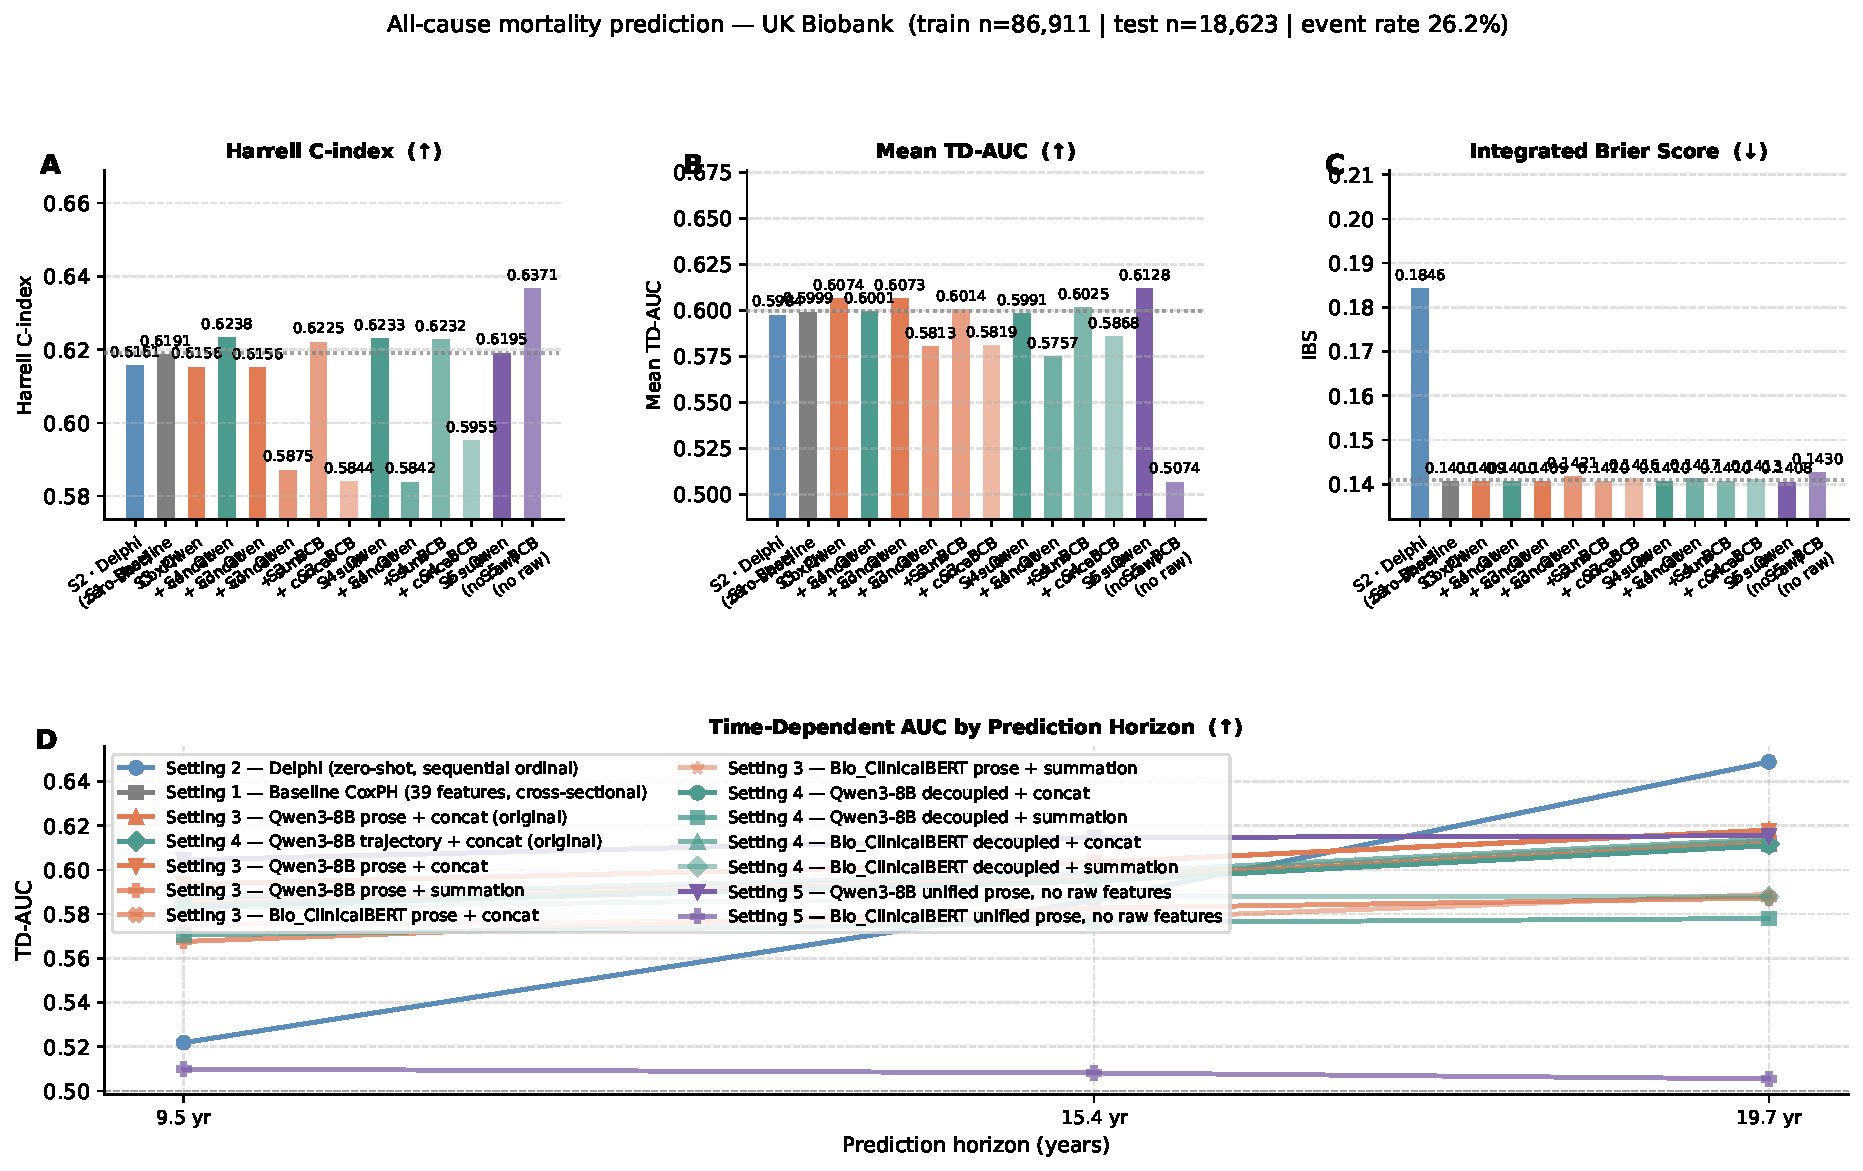
\includegraphics[width=\textwidth]{figures/figure_main}
  \caption{Test-set performance for the five input-format settings (Axis A,
           reference configurations).
           (A) Harrell C-index with the cross-sectional baseline (S1) as dotted reference;
           (B) mean time-dependent AUC; (C) Integrated Brier Score;
           (D) TD-AUC by prediction horizon.
           All embedding variants use Qwen3-Embedding (8B) as the encoder and
           concatenation fusion where applicable.}
  \label{fig:results}
\end{figure}
